
\section{Introduction}

Data partitioning strategy was originally studied in a shared-memory
environment, where XML data is stored in a shared memory and can be concurrently
accessible by multiple XPath processors. In the conclusion of the original
paper,  the author had pointed out that the parallelization model is over XML
data model, it  can be adapted to any XML storage laryout. However, no matter in
the original study,  or in our previous study, the strategies are applied both
in a shared-memory environment. Therefore, here comes a question:  how we can
apply it in a distributed-memory environment? In this study, by exploiting
horizontal fragmentation on XML data, we present our study on applying data
partitioning in a distributed-memory environment to experimentally show how it
improves the scalability.

\section{Fragmentation}

Fragmentation is an effective way to improve scalability of database
systems~\cite{navathe1995mixed, hauglid2010dyfram, khan2010new}.  In the field
of parallel XML processing, there are also some studies on  fragmentation of XML
data~\cite{kling11:dist_xml, KlOD10}.  The most common XML fragmentations are
horizontal fragmentation and vertical fragmentation~\cite{kling11:dist_xml}. Due
to the nature of horizontal fragments that are  relatively independent, it is a
more direct and practical way to work together with data partitioning. We thus
focus on only horizontal fragmentation in this study.

We first define horizontal fragmentation.  Let $D$ = \{$d_1$, $d_2$, ...,
$d_n$\} be a collection of document trees such that each $d_i \in D$ conforms
the same XML schema~\cite{xmlschema}.  Let $\mathit{FS}$ = \{$F_1$, $F_2$,...,
$F_m$\}  be a collection of fragments such that for each $F_i \subset D$. If
$\bigcup\limits_{i=1}^{m} F_{i} = F$ and $\bigcap\limits_{i=1}^{m} F_{i} =
\emptyset$, then $\mathit{FS}$ is a horizontal fragmentation of $D$.

Let us take the tree in Fig.~\ref{fig:hfrag_example} as an example. There are
five document trees in Fig.~\ref{fig:hfrag_example}(a), i.e. we have $D$ =
\{$d_1$, $d_2$, $d_3$, $d_4$, $d_5$\}, where $d_1$ is  the first subtree rooted
at $b$ (from left to right), $d_2$ be the second and so on. All the subtrees
follow the schema in Fig.~\ref{fig:hfrag_example}(b). We can make three
horizontal fragments $FS$ = \{$F_1$, $F_2$, $F_3$\} as shown in the three dotted
rectangles, where $F_1$ = \{$d_1$, $d_2$\}, $F_2$ = \{$d_3$\} and  $F_3$ =
\{$d_4$, $d_5$\}.


\begin{figure}[t]
	\centering
	\begin{subfigure}{.6\textwidth}
		\centering
		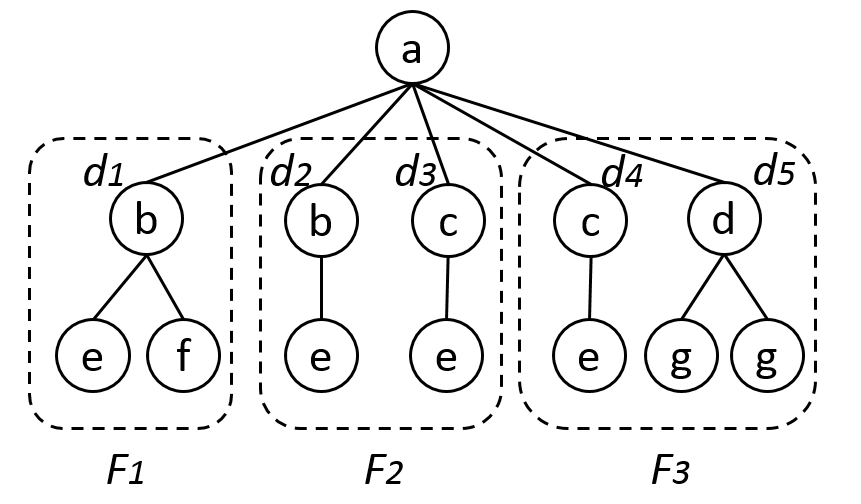
\includegraphics[width=.99\linewidth]{figures/hfrag_example}
		\caption{An example of horizontal fragmentation}
		\label{fig:sub1}
	\end{subfigure}%
	\begin{subfigure}{.4\textwidth}
		\centering
		\vspace{12mm}
		\begin{tabular}{|l|}
			\hline
			schema\\
			\hline
			a(b*, c*, d) \\
			b(e, f?) \\
			c(e) \\
			d(g*) \\
			\hline
		\end{tabular}
		\vspace{12mm}
		\caption{The schema of the example}
		\label{fig:sub2}
	\end{subfigure}
	\caption{An example of horizontal fragmentation and the schema.}
	\label{fig:hfrag_example}
\end{figure}



\section{Our Ditributed XPath Query Framework}

We design an XPath query framework using horizontal fragmentation with data
partitioning strategy on top of BaseX over a distributed-memory environment. 
The implementation consists of the following four stages:\\
\begin{itemize}
	\item Data Fragmentation \\To divide an input XML document into fragments.
	\item Allocation\\ To assign the fragments into multiple computation nodes.
	\item Query Evaluation\\ To query fragments in parallel
	\item Results Merging\\ To merge the results of fragents to form the final result.
\end{itemize}

We give the detailed introduction in the following sections.

\subsection{Fragmentation}

In our framework, we first apply horizontal fragmentation to the input XML data,
through which an XML tree is divided into a set of fragments. To make the 
fragmentation works well in combination with data partitioning strategy. We
have the following requirements.

\subsubsection{Fragments are size-balanced}

Since the mainpurpose of fragmentation is to achieve good scalability, we
attempt to make our fragmentation algorithm size-balanced, i.e. to make each
fragment have nearly the same amount of node. 

\subsubsection{Path to the root is added}

In our design desire of fragmentation algorithm, we also intent to ease the
querying. Thus, we require that each fragment is a set of consecutive
sibling subtrees augmented with the path to the root. Note that two
subtrees are sibling subtrees if the roots of the subtrees are siblings of each
other.

\subsubsection{Correctness}

We assume that all the results lie in the subtrees on the fragment. Thus,
to guarantee the correctness of query results, we need to guarantee the
completeness and uniqueness of nodes such that each node in the input XML tree
is included in at least a fragment. If a node is included a subtree part of a
fragment, then it is not included in any other fragment.


\begin{figure}[]
	\centering
	\begin{tabular}{l}
		\hline
		\hline
		\makebox[.95\linewidth][l]{\textbf{Algorithm 1} \textsc{Fragmentation}($\mathit{nodes}$, $\mathit{MAXSIZE}$)} \\
		\hline
		\textbf{Input}:           $\mathit{nodes}$: a list of nodes, \\
		\makebox[1em][r]{}\hspace{9 mm}  $\mathit{MAXSIZE} $ : the maximum number of nodes in a fragment \\
		\textbf{Output}: a list of fragments \\
		\makebox[1em][r]{1:}\hspace{1 mm}  $\mathit{fragments} \leftarrow [] $     //a list of fragments \\
		\makebox[1em][r]{2:}\hspace{1 mm}  $subtrees \leftarrow [] $     //a list of root nodes of subtrees \\
		\makebox[1em][r]{3:}\hspace{1 mm}  \textbf{for all} $\emph{node} \in \emph{nodes}$ \textbf{do} \\
		\makebox[1em][r]{4:}\hspace{5 mm}  \textbf{if} \texttt{size($node$)} $ > \mathit{MAXSIZE} $ \textbf{then} \\
		\makebox[1em][r]{5:}\hspace{9 mm}  \textbf{if} $subtrees.length > 0$  \textbf{then} \\
		\makebox[1em][r]{6:}\hspace{13 mm} $\mathit{fragments}.Add((\textit{\_, subtrees}))$ \\
		\makebox[1em][r]{7:}\hspace{13 mm}  $\mathit{subtrees} \leftarrow []$ \\
		\makebox[1em][r]{8:}\hspace{9 mm}  \textbf{end if}\\
		\makebox[1em][r]{9:}\hspace{9 mm}  $\mathit{fragments}.AddAll($\texttt{Fragmentation}$($\texttt{child}$(node), \mathit{MAXSIZE}))$ \\
		\makebox[1em][r]{10:}\hspace{5 mm}  \textbf{else if} \texttt{size($node$)} + \texttt{Size}$(subtrees) > \mathit{MAXSIZE}$ \textbf{then} \\
		\makebox[1em][r]{11:}\hspace{9 mm} $\mathit{fragments}.Add((\_, subtrees))$ \\
		\makebox[1em][r]{12:}\hspace{9 mm} $subtrees \leftarrow [node]$ \\
		\makebox[1em][r]{13:}\hspace{5 mm}  \textbf{else}\\
		\makebox[1em][r]{14:}\hspace{9 mm} $\mathit{subtrees}.Add(node)$ \\
		\makebox[1em][r]{15:}\hspace{5 mm}  \textbf{end if}\\
		\makebox[1em][r]{16:}\hspace{1 mm}  \textbf{end for}\\
		\makebox[1em][r]{17:}\hspace{1 mm}  \textbf{for} $i \in [0, \mathit{fragments}.length)$ \textbf{do}\\
		\makebox[1em][r]{18:}\hspace{5 mm}  $\mathit{fragments}[i] \leftarrow $\texttt{AddPath}($\mathit{fragments}[i]$)  \\
		\makebox[1em][r]{19:}\hspace{1 mm}  \textbf{end for}\\
		\makebox[1em][r]{20:}\hspace{1 mm}  \textbf{return} $\mathit{fragments}$\\
		\hline
	\end{tabular}
	\caption{The fragmentation algorithm.}
	\label{fig:algQuery1}
\end{figure}


\begin{figure}[]
	\centering
	\begin{tabular}{l}
		\hline
		\hline
		\makebox[.95\linewidth][l]{\textbf{Algorithm 2} \textsc{AddPath}($\mathit{subtrees}$)} \\
		\hline
		\textbf{Input}:   $\mathit{subtrees}$: a list of root nodes of subtrees \\
		\textbf{Output}:  the root node of a tree that is augmented with the \\
		\makebox[1em][r]{}\hspace{13 mm}  path to the root of the whole tree\\
		\makebox[1em][r]{1:}\hspace{1 mm}  $\mathit{p} \leftarrow $\texttt{parent}$(subtrees[0]) $   \\
		\makebox[1em][r]{2:}\hspace{1 mm}  $node \leftarrow $ \texttt{clone}($p$)    \\
		\makebox[1em][r]{3:}\hspace{1 mm}  $node.addChildren(subtrees) $ \\
		\makebox[1em][r]{4:}\hspace{1 mm}  \textbf{while} \texttt{parent}$(p) \neq \mathit{NULL}$ \textbf{do}\\
		\makebox[1em][r]{5:}\hspace{5 mm}  $p \leftarrow $ \texttt{parent}($p$) \\
		\makebox[1em][r]{6:}\hspace{5 mm}  $tempnode \leftarrow$ \texttt{clone}($p$)  \\
		\makebox[1em][r]{7:}\hspace{5 mm}  $tempnode.addChild(node)$ \\
		\makebox[1em][r]{8:}\hspace{5 mm}  $node \leftarrow tempnode$ \\
		\makebox[1em][r]{9:}\hspace{1 mm}  \textbf{end while} \\
		\makebox[1em][r]{10:}\hspace{1 mm}  \textbf{return} $\mathit{node}$\\
		\hline
	\end{tabular}
	\caption{Add path to a list of subtrees}
	\label{fig:algQuery2}
\end{figure}

\begin{figure}[!t] 
	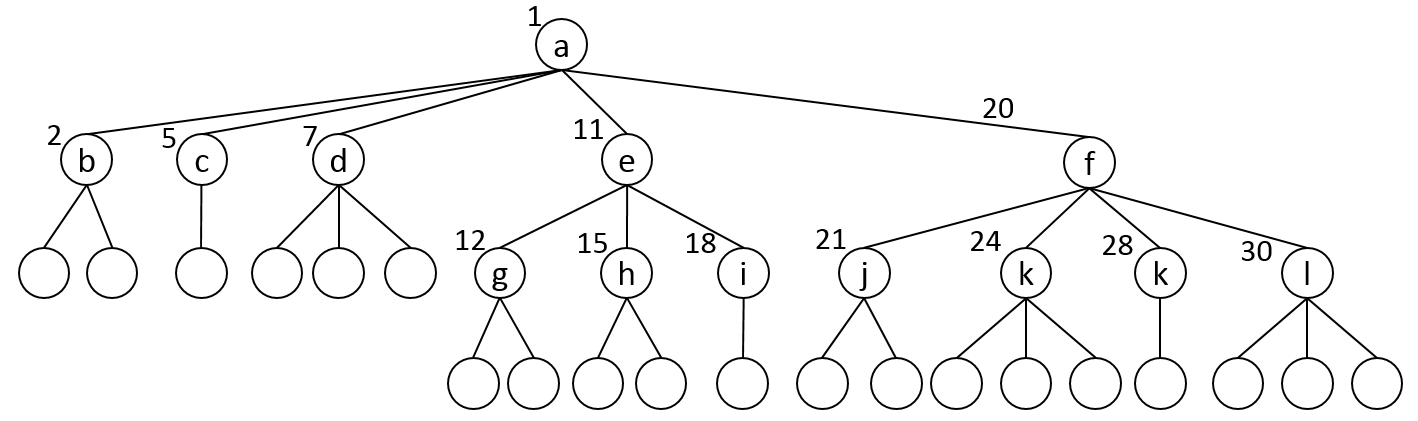
\includegraphics[scale=0.38]{basex/figures/fragment1}
	\caption{An example tree with number denoting PRE values of nodes}
	\label{fig:frag1}
	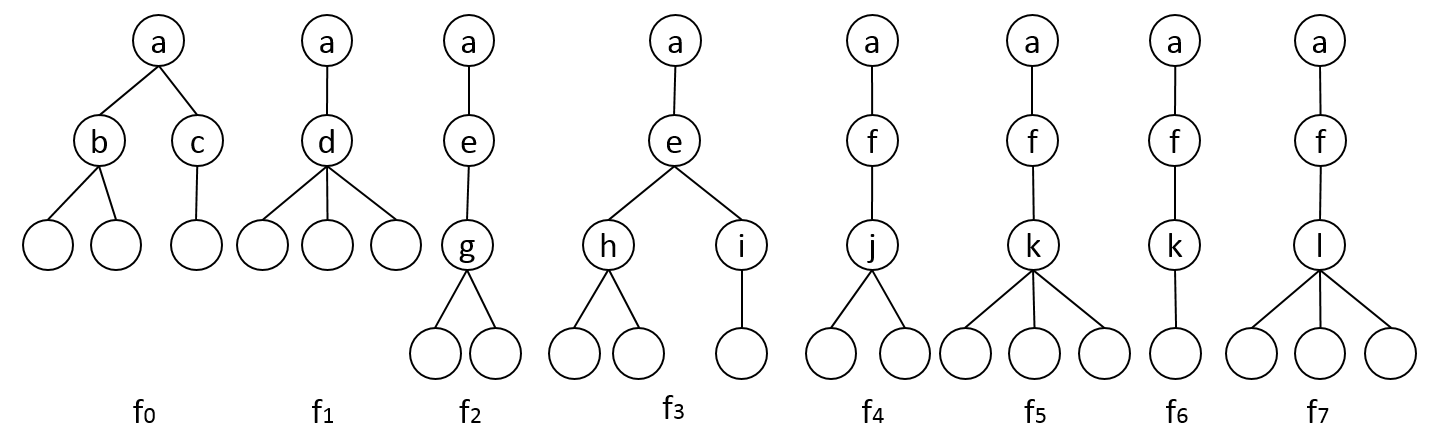
\includegraphics[scale=0.38]{basex/figures/fragment2}
	\caption{Recontructed fragments.}
	\label{fig:frag2}
	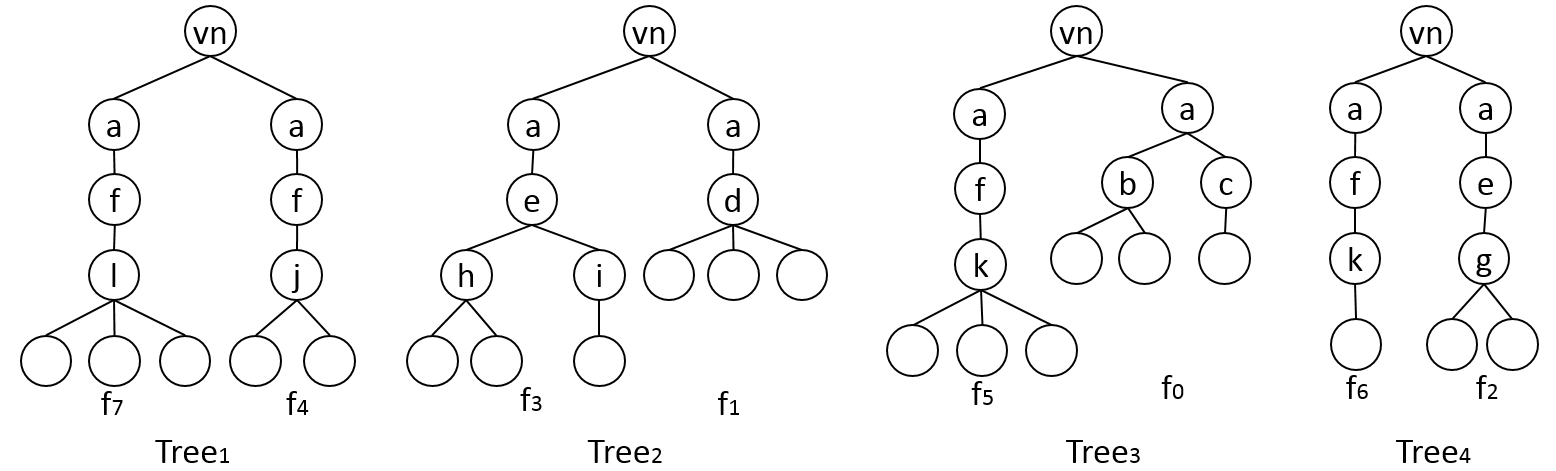
\includegraphics[scale=0.35]{basex/figures/fragment3}
	\caption{Regroup and merge.}
	\label{fig:frag3}
\end{figure}



Algorithm 1 describes how our fragmentation works to apply a horizontal
fragmentation to a tree. The arguments of input are a list of nodes denoting the
tree to be fragmented and an integer number denoting the maximum number of nodes
a fragment can have so that we can make the fragments in similar size.   In Line
1--2, we declare an empty list of fragments and an empty list of subtrees for
holding results. In Line 3--16, we traverse each node in the input list, if the
node have more number of descendant nodes greater than MAXSIZE, we apply the
fragmentation on the children of the node (Line 4--9) and add the results into
$fragments$. Else if total number of descendant nodes in $subtrees$ and the
$node$ excesses MAXSIZE, we save the current fragment and put the current node
into a new fragment (Line 10--12). Otherwise, the current node is added to
$subtrees$ as one of the subtrees in the current fragment. After the iteration,
we obtain a list of fragments, each of which is a list of subtrees. We add the
last use Algorithms 2 to complete each fragment by adding the path from the
current subtrees to the root of the original tree (Line 17--19). In Algorithm 2,
we basically keep looking upward, to add all the ancestor nodes to the current
fragment.

There are also several functions used in Algorithms 1 and 2 that are described 
as below:\\
- \texttt{size($node$)} returns the number of descendants of $node$, where node
is a single node.\\
- \texttt{Size($nodes$)} returns the sum of number of descendants of each node
in $nodes$, where $nodes$ is a list of nodes.\\
- \texttt{child($node$)} returns the children of $node$.
- \texttt{parent($node$)} returns the parent of $node$.\\
- \texttt{clone($node$)} returns a node cloned from $node$. The function create
an empty node and copy the name and attributes from $node$.

Note that for the query processing, we need a representative value for each
fragment to maintain the original order of a fragment as in the original tree.
We simply use a fragment id for each fragment.

Let us take the tree shown in Fig.~\ref{fig:frag1} as an example with MAXSIZE =
3. After Line 16 of Algorithm 1, the fragments are list of subtrees. When we use
the PRE index to denote the root node of a subtree, we have F = [f$_1$, f$_2$, ...,
f$_8$] = [[2, 5], [7], [12], [15, 18], [21], [24], [28], [30]], where the
subscripted numbers are the fragment ids. Then, by applying Algorithm 2 that adds
the path from the subtrees to the root of the whole tree, we obtain the final
recontructed fragment as shown in Fig.~\ref{fig:frag2}.

\subsection{Allocation}

After fragmentation, the fragments are mapped to multiple computation nodes. For each
computation node, a sub set of fragments is assigned. To make the distribution
of fragments well-balanced, we randomly shuffle the list of fragments before
dividing the list into $N$ lists of fragments, where N is the same as the number
of computation nodes. 

We use a mapping list to map the fragments. An element in the mapping list
contains information for locating the corresponding fragment so that we can
access and process query on the fragment independently.  With this mapping list,
we can start a query by locating the root of each fragment on any tree, making
it possible to evaluate queries on them in parallel.  And also, the mapping list
can be used to maintain the order of results to form the final results.

In our study, we run a single BaseX instance in server mode on each computation
node. For each computation node, the sub set of fragments on it is then added to
an empty root node to form a complete XML tree so that we can load the tree by
the BaseX server to create an XML database for further query evaluation. To make
each list of fragments become a single tree (so that we can create a database in
BaseX from it),  we create a node as the root and add the lists of the fragments
to the root, where the root of a fragment becomes the child of the newly added
root node. 

Let us continue the running example. Let N be 4, after shuffling and regrouping,
we may obtain four groups of fragments: FS $=>$ [F$_1$, F$_2$, F$_3$, F$_4$], where
F$_1$ = [$f_7$, $f_4$],
F$_2$ = [$f_3$, $f_1$],
F$_3$ = [$f_5$, $f_0$],
F$_4$ = [$f_6$, $f_2$].
By adding a root node $vn$ to the each group, we create four trees from FS
respectively as shown in Fig.~\ref{fig:frag3}.

We also create a mapping list of links $links$ for each F in FS for locating.
A link is a 3-tuple ($Tree,
pre, depth$), where $tree$ is a pointer to a reconstructed tree, $pre$ is the PRE
value of the root of a fragment in $tree$, $depth$ is the number of nodes in the
path from subtrees to the root. For the given example, we have a list of links
$links$ =
[(Tree$_3$, 2, 1),
(Tree$_2$, 9, 1),
(Tree$_4$, 6, 2),
(Tree$_2$, 2, 2),
(Tree$_1$, 8, 2),
(Tree$_3$, 2, 2),
(Tree$_4$, 2, 2),
(Tree$_1$, 2, 2)],
where $links[0] \rightarrow f_0$, $links[1] \rightarrow f_1$, ...,  $links[7]
\rightarrow f_7$.

\subsection{Query evaluation}

In our implementation on top of BaseX, each of fragment has already been
inserted into BaseX server on a computation node as a database before querying.
By using the mapping list $links$, we perform a given query on the databases in
parallel using multiple cores by using \texttt{db:open-pre(`db', pre)} function
on top of BaseX. We may apply data partitioning strategy on a single fragment,
or compute in parallel over multiple fragments.

Let us take $links[0] = ($Tree$_3, 2) \rightarrow f_0$ as an example. We start
the query from the root node of $f_0$ located in Tree$_3$. In the implementation
on top of BaseX, we use \texttt{db:open-pre(`db', pre)} to locate a node with
PRE value \texttt{pre} in a database namely \texttt{db}. In this example,
\texttt{db} corresponds the database created from Tree$_3$, and \texttt{pre} is
2. Let the name of the database be \texttt{xmark40\_0} and the query be
\texttt{/site//open\_auction//bidder[last()]}, We can evaluate the query from
the root of $f_0$ as \\ \texttt{db:open-pre(`xmark40\_0',
	2)//open\_auction//bidder[last()]}\\ Note that, since
\texttt{db:open-pre(`xmark40\_0', 2)} is the root \texttt{site}, we removed
\texttt{/site} in the expression.

We can also can apply the server-side implementation of DPS to the fragment. The
example query can be rewritten into a prefix query $prefix$ =
\texttt{//open\_auction} and a suffix query $suffix$ = \texttt{bidder[last()]}.
The application of DPS is basically the same as the original way. The only
difference is where to start the prefix query. In this case, we use
\texttt{db:open-pre(`db', pre)prefix} to start the prefix query instead of
\texttt{db:open(`db')prefix}. Note that $depth$ can be used to help the
rewritting of query. The partitioning place in the query should be at level
greater than $depth$, otherwize there will be only 1 node in the result of
prefix query. Also, we omit \texttt{/site} as mentioned above.


\subsection{Results Merging}

Last, the results received from BaseX servers on computation nodes are collected
and merged to form the final result. We evaluate all fragments in parallel by
using $links$. After the evaluation of each fragment is done, we merge the
results from each link in the same order as it in the $links$. For our example,
we simply merge the results by concatenating the result of $f_0$ through the
result of $f_7$.


\section{Experiments}

For the experiment part, I decide to use 4 computers, each has 4 cores
(matsu-lab50--matsu-lab53). The XMark dataset sizes 4.4 GB with 66.65M nodes.
The MAXSIZE is set to 4.2M, so that we can divide the dataset into 16 fragments
(my intention is to assign one to each core). I use two settings for
experiments. One that only runs queries in parallel and the another also applies
to data partitioning strategy. We will compare the two setting to show how much
DPS can be used to improve the query efficiency.

